

% BOILERPLATE - Allows for individual chapters to be compiled.
%
% Usage:
%    % BOILERPLATE - Allows for individual chapters to be compiled.
%
% Usage:
%    % BOILERPLATE - Allows for individual chapters to be compiled.
%
% Usage:
%    \input{../settings/boilerplate} % place at start and end of chapter
% 

\def\precommands{%
    \input{../settings/phdsetup}
    \def\preinserted{}
    \begin{document}
}

\def\postcommands{%
    \singlespacing
    \phantomsection
%    \bibliographystyle{../bibliography/expanded}
   \bibliographystyle{elsarticle-harv}
   \bibliography{../bibliography/references}
    \enddocument
}

\def\autoinsert{%
    \ifx\preinserted\undefined
        \expandafter\precommands
    \else
        \expandafter\postcommands
    \fi
}

\ifx\master\undefined\expandafter\autoinsert\fi

 % place at start and end of chapter
% 

\def\precommands{%
    % [ USER VARIABLES ]

\def\PHDTITLE {Regime shifts in ecology and evolution}
\def\PHDAUTHOR{Carl Boettiger}
\def\PHDSCHOOL{University of California, Davis}

\def\PHDMONTH {September}
\def\PHDYEAR  {2012}
\def\PHDDEPT {Center for Population Biology}

\def\BSSCHOOL {Princeton}
\def\BSYEAR   {2007}

\def\PHDCOMMITTEEA{Alan Hastings}
\def\PHDCOMMITTEEB{Peter Wainwright}
\def\PHDCOMMITTEEC{Brian Moore}

% [ GLOBAL SETUP ]

\documentclass[letterpaper,oneside,11pt]{report}


% [ CARL BOETTIGER`S CUSTOM COMMANDS, LIBRARIES, ETC ]

\usepackage{subfigure}
\usepackage[sort&compress]{natbib}
\usepackage{color}
\usepackage{fancyvrb}
\usepackage{ctable}


\usepackage{silence}
\WarningFilter{amsmath}{Underfull}     

%\newcommand{\argmax}{\operatorname{argmax}}
\newcommand{\ud}{\mathrm{d}}


\usepackage{calc}
\usepackage{breakcites}
\usepackage[newcommands]{ragged2e}
\usepackage{appendix}
\usepackage{comment}
\usepackage{xifthen}

\usepackage{graphicx}
\usepackage{epstopdf}


\renewenvironment{abstract}{\chapter*{Abstract}}{}
\renewcommand{\bibname}{Bibliography}
\renewcommand{\contentsname}{Table of Contents}

\makeatletter
\renewcommand{\@biblabel}[1]{\textsc{#1}}
\makeatother

% [ FONT SETTINGS ]

\usepackage[T1]{fontenc}
\usepackage{libertine}

\usepackage[tbtags, intlimits, namelimits]{amsmath}
\usepackage{amsthm}
\usepackage{amssymb}
\usepackage{amsfonts}



% [ PAGE LAYOUT ]

\usepackage{geometry}
\geometry{lmargin = 1.5in}
\geometry{rmargin = 1.0in}
\geometry{tmargin = 1.0in}
\geometry{bmargin = 1.0in}

% [ PDF SETTINGS ]

\usepackage[final]{hyperref}
\hypersetup{
    breaklinks  = {true},
    colorlinks  = {true},
    linktocpage = {false},
    linkcolor   = {blue},
    citecolor   = {black},
    urlcolor    = {black},
    plainpages  = {false},
    pageanchor  = {true},
    pdfauthor   = {\PHDAUTHOR},
    pdftitle    = {\PHDTITLE},
    pdfsubject  = {Dissertation, \PHDSCHOOL},
    pdfcreator  = {},
    pdfkeywords = {},
    pdfproducer = {}
}
\urlstyle{same}

% [ LETTER SPACING ]

\usepackage[final]{microtype}
\microtypesetup{protrusion=compatibility}
\microtypesetup{expansion=false}

\newcommand{\upper}[1]{\MakeUppercase{#1}}
\let\lsscshape\scshape

\ifcase\pdfoutput\else\microtypesetup{letterspace=15}
\renewcommand{\scshape}{\lsscshape\lsstyle}
\renewcommand{\upper}[1]{\textls[50]{\MakeUppercase{#1}}}\fi

% [ LINE SPACING ]

\usepackage[doublespacing]{setspace}
\renewcommand{\displayskipstretch}{0.75}

\setlength{\parskip   }{0em}
\setlength{\parindent }{2em}

% [ TABLE FORMATTING ]

\usepackage{booktabs}
\usepackage{multirow}
\usepackage{dcolumn}
\setlength{\heavyrulewidth}{1.5\arrayrulewidth}
\setlength{\lightrulewidth}{1.0\arrayrulewidth}
\setlength{\doublerulesep }{2.0\arrayrulewidth}

% [ SECTION FORMATTING ]

\usepackage[largestsep,nobottomtitles*]{titlesec}
\renewcommand{\bottomtitlespace}{0.75in}

\titleformat{\chapter}[display]%
    {\bfseries\huge\singlespacing}%
    {\filleft\textsc{\LARGE \chaptertitlename\ \thechapter}}%
    {-0.2ex}{\titlerule[3pt]\vspace{0.2ex}}[]

\titleformat{\section}{\LARGE}{\thesection\hspace{0.5em}}{0ex}{}
\titleformat{\subsection}{\Large}{\thesubsection\hspace{0.5em}}{0ex}{}
\titleformat{\subsubsection}{\large}{\thesubsubsection\hspace{0.5em}}{0ex}{}

\titlespacing*{\chapter}{0em}{6ex}{4ex plus 2ex minus 0ex}
\titlespacing*{\section}{0em}{2ex plus 3ex minus 1ex}{0.5ex plus 0.5ex minus 0.5ex}
\titlespacing*{\subsection}{0ex}{2ex plus 3ex minus 1ex}{0ex}
\titlespacing*{\subsubsection}{0ex}{2ex plus 0ex minus 1ex}{0ex}

% [ HEADER SETTINGS ]

\usepackage{fancyhdr}

\setlength{\headheight}{\normalbaselineskip}
\setlength{\footskip  }{0.5in}
\setlength{\headsep   }{0.5in-\headheight}

\fancyheadoffset[R]{0.5in}
\renewcommand{\headrulewidth}{0pt}
\renewcommand{\footrulewidth}{0pt}

\newcommand{\pagebox}{\parbox[r][\headheight][t]{0.5in}{\hspace\fill\thepage}}

\newcommand{\prelimheaders}{\ifx\prelim\undefined\renewcommand{\thepage}{\textit{\roman{page}}}\fancypagestyle{plain}{\fancyhf{}\fancyfoot[L]{\makebox[\textwidth-0.5in]{\thepage}}}\pagestyle{plain}\def\prelim{}\fi}

\newcommand{\normalheaders}{\renewcommand{\thepage}{\arabic{page}}\fancypagestyle{plain}{\fancyhf{}\fancyhead[R]{\pagebox}}\pagestyle{plain}}

\normalheaders{}

% [ CUSTOM COMMANDS ]

\newcommand{\signaturebox}[1]{\multicolumn{1}{p{4in}}{\vspace{3ex}}\\\midrule #1\\}

% Redefine AMS proof environment to have itshape
% Note: This environment automatically adds \qed at the end. If your proof
% ends in a math environment, the \qed is placed, undesirably, on a new line.
% To prevent that, insert \qedhere inside the math environment.
\makeatletter
\renewenvironment{proof}[1][\proofname]{%
\par\pushQED{\qed}\normalfont%
\topsep6\p@\@plus6\p@\relax\trivlist%
\item[\hskip\labelsep\bfseries#1\@addpunct{.}]\itshape\ignorespaces}{%
\popQED\endtrivlist\@endpefalse}%
\makeatother

% TUGboat, Volume 0 (2001), No. 0
% http://math.arizona.edu/~aprl/publications/mathclap/perlis_mathclap_24Jun2003.pdf
% For comparison, here are the existing overlap macros:
% \def\llap#1{\hbox to 0pt{\hss#1}}
% \def\rlap#1{\hbox to 0pt{#1\hss}}
\def\clap#1{\hbox to 0pt{\hss#1\hss}}
\def\mathllap{\mathpalette\mathllapinternal}
\def\mathrlap{\mathpalette\mathrlapinternal}
\def\mathclap{\mathpalette\mathclapinternal}
\def\mathllapinternal#1#2{%
\llap{$\mathsurround=0pt#1{#2}$}}
\def\mathrlapinternal#1#2{%
\rlap{$\mathsurround=0pt#1{#2}$}}
\def\mathclapinternal#1#2{%
\clap{$\mathsurround=0pt#1{#2}$}}

\newcommand{\alert}[1]{\textbf{\textcolor{red}{#1}}}




% [ Code blocks ]
%\DefineShortVerb[commandchars=\\\{\}]{\|}
\DefineVerbatimEnvironment{Highlighting}{Verbatim}{commandchars=\\\{\}}
% Add ',fontsize=\small' for more characters per line
\newenvironment{Shaded}{}{}
\newcommand{\KeywordTok}[1]{\textcolor[rgb]{0.00,0.44,0.13}{\textbf{{#1}}}}
\newcommand{\DataTypeTok}[1]{\textcolor[rgb]{0.56,0.13,0.00}{{#1}}}
\newcommand{\DecValTok}[1]{\textcolor[rgb]{0.25,0.63,0.44}{{#1}}}
\newcommand{\BaseNTok}[1]{\textcolor[rgb]{0.25,0.63,0.44}{{#1}}}
\newcommand{\FloatTok}[1]{\textcolor[rgb]{0.25,0.63,0.44}{{#1}}}
\newcommand{\CharTok}[1]{\textcolor[rgb]{0.25,0.44,0.63}{{#1}}}
\newcommand{\StringTok}[1]{\textcolor[rgb]{0.25,0.44,0.63}{{#1}}}
\newcommand{\CommentTok}[1]{\textcolor[rgb]{0.38,0.63,0.69}{\textit{{#1}}}}
\newcommand{\OtherTok}[1]{\textcolor[rgb]{0.00,0.44,0.13}{{#1}}}
\newcommand{\AlertTok}[1]{\textcolor[rgb]{1.00,0.00,0.00}{\textbf{{#1}}}}
\newcommand{\FunctionTok}[1]{\textcolor[rgb]{0.02,0.16,0.49}{{#1}}}
\newcommand{\RegionMarkerTok}[1]{{#1}}
\newcommand{\ErrorTok}[1]{\textcolor[rgb]{1.00,0.00,0.00}{\textbf{{#1}}}}
\newcommand{\NormalTok}[1]{{#1}}



    \def\preinserted{}
    \begin{document}
}

\def\postcommands{%
    \singlespacing
    \phantomsection
%    \bibliographystyle{../bibliography/expanded}
   \bibliographystyle{elsarticle-harv}
   \bibliography{../bibliography/references}
    \enddocument
}

\def\autoinsert{%
    \ifx\preinserted\undefined
        \expandafter\precommands
    \else
        \expandafter\postcommands
    \fi
}

\ifx\master\undefined\expandafter\autoinsert\fi

 % place at start and end of chapter
% 

\def\precommands{%
    % [ USER VARIABLES ]

\def\PHDTITLE {Regime shifts in ecology and evolution}
\def\PHDAUTHOR{Carl Boettiger}
\def\PHDSCHOOL{University of California, Davis}

\def\PHDMONTH {September}
\def\PHDYEAR  {2012}
\def\PHDDEPT {Center for Population Biology}

\def\BSSCHOOL {Princeton}
\def\BSYEAR   {2007}

\def\PHDCOMMITTEEA{Alan Hastings}
\def\PHDCOMMITTEEB{Peter Wainwright}
\def\PHDCOMMITTEEC{Brian Moore}

% [ GLOBAL SETUP ]

\documentclass[letterpaper,oneside,11pt]{report}


% [ CARL BOETTIGER`S CUSTOM COMMANDS, LIBRARIES, ETC ]

\usepackage{subfigure}
\usepackage[sort&compress]{natbib}
\usepackage{color}
\usepackage{fancyvrb}
\usepackage{ctable}


\usepackage{silence}
\WarningFilter{amsmath}{Underfull}     

%\newcommand{\argmax}{\operatorname{argmax}}
\newcommand{\ud}{\mathrm{d}}


\usepackage{calc}
\usepackage{breakcites}
\usepackage[newcommands]{ragged2e}
\usepackage{appendix}
\usepackage{comment}
\usepackage{xifthen}

\usepackage{graphicx}
\usepackage{epstopdf}


\renewenvironment{abstract}{\chapter*{Abstract}}{}
\renewcommand{\bibname}{Bibliography}
\renewcommand{\contentsname}{Table of Contents}

\makeatletter
\renewcommand{\@biblabel}[1]{\textsc{#1}}
\makeatother

% [ FONT SETTINGS ]

\usepackage[T1]{fontenc}
\usepackage{libertine}

\usepackage[tbtags, intlimits, namelimits]{amsmath}
\usepackage{amsthm}
\usepackage{amssymb}
\usepackage{amsfonts}



% [ PAGE LAYOUT ]

\usepackage{geometry}
\geometry{lmargin = 1.5in}
\geometry{rmargin = 1.0in}
\geometry{tmargin = 1.0in}
\geometry{bmargin = 1.0in}

% [ PDF SETTINGS ]

\usepackage[final]{hyperref}
\hypersetup{
    breaklinks  = {true},
    colorlinks  = {true},
    linktocpage = {false},
    linkcolor   = {blue},
    citecolor   = {black},
    urlcolor    = {black},
    plainpages  = {false},
    pageanchor  = {true},
    pdfauthor   = {\PHDAUTHOR},
    pdftitle    = {\PHDTITLE},
    pdfsubject  = {Dissertation, \PHDSCHOOL},
    pdfcreator  = {},
    pdfkeywords = {},
    pdfproducer = {}
}
\urlstyle{same}

% [ LETTER SPACING ]

\usepackage[final]{microtype}
\microtypesetup{protrusion=compatibility}
\microtypesetup{expansion=false}

\newcommand{\upper}[1]{\MakeUppercase{#1}}
\let\lsscshape\scshape

\ifcase\pdfoutput\else\microtypesetup{letterspace=15}
\renewcommand{\scshape}{\lsscshape\lsstyle}
\renewcommand{\upper}[1]{\textls[50]{\MakeUppercase{#1}}}\fi

% [ LINE SPACING ]

\usepackage[doublespacing]{setspace}
\renewcommand{\displayskipstretch}{0.75}

\setlength{\parskip   }{0em}
\setlength{\parindent }{2em}

% [ TABLE FORMATTING ]

\usepackage{booktabs}
\usepackage{multirow}
\usepackage{dcolumn}
\setlength{\heavyrulewidth}{1.5\arrayrulewidth}
\setlength{\lightrulewidth}{1.0\arrayrulewidth}
\setlength{\doublerulesep }{2.0\arrayrulewidth}

% [ SECTION FORMATTING ]

\usepackage[largestsep,nobottomtitles*]{titlesec}
\renewcommand{\bottomtitlespace}{0.75in}

\titleformat{\chapter}[display]%
    {\bfseries\huge\singlespacing}%
    {\filleft\textsc{\LARGE \chaptertitlename\ \thechapter}}%
    {-0.2ex}{\titlerule[3pt]\vspace{0.2ex}}[]

\titleformat{\section}{\LARGE}{\thesection\hspace{0.5em}}{0ex}{}
\titleformat{\subsection}{\Large}{\thesubsection\hspace{0.5em}}{0ex}{}
\titleformat{\subsubsection}{\large}{\thesubsubsection\hspace{0.5em}}{0ex}{}

\titlespacing*{\chapter}{0em}{6ex}{4ex plus 2ex minus 0ex}
\titlespacing*{\section}{0em}{2ex plus 3ex minus 1ex}{0.5ex plus 0.5ex minus 0.5ex}
\titlespacing*{\subsection}{0ex}{2ex plus 3ex minus 1ex}{0ex}
\titlespacing*{\subsubsection}{0ex}{2ex plus 0ex minus 1ex}{0ex}

% [ HEADER SETTINGS ]

\usepackage{fancyhdr}

\setlength{\headheight}{\normalbaselineskip}
\setlength{\footskip  }{0.5in}
\setlength{\headsep   }{0.5in-\headheight}

\fancyheadoffset[R]{0.5in}
\renewcommand{\headrulewidth}{0pt}
\renewcommand{\footrulewidth}{0pt}

\newcommand{\pagebox}{\parbox[r][\headheight][t]{0.5in}{\hspace\fill\thepage}}

\newcommand{\prelimheaders}{\ifx\prelim\undefined\renewcommand{\thepage}{\textit{\roman{page}}}\fancypagestyle{plain}{\fancyhf{}\fancyfoot[L]{\makebox[\textwidth-0.5in]{\thepage}}}\pagestyle{plain}\def\prelim{}\fi}

\newcommand{\normalheaders}{\renewcommand{\thepage}{\arabic{page}}\fancypagestyle{plain}{\fancyhf{}\fancyhead[R]{\pagebox}}\pagestyle{plain}}

\normalheaders{}

% [ CUSTOM COMMANDS ]

\newcommand{\signaturebox}[1]{\multicolumn{1}{p{4in}}{\vspace{3ex}}\\\midrule #1\\}

% Redefine AMS proof environment to have itshape
% Note: This environment automatically adds \qed at the end. If your proof
% ends in a math environment, the \qed is placed, undesirably, on a new line.
% To prevent that, insert \qedhere inside the math environment.
\makeatletter
\renewenvironment{proof}[1][\proofname]{%
\par\pushQED{\qed}\normalfont%
\topsep6\p@\@plus6\p@\relax\trivlist%
\item[\hskip\labelsep\bfseries#1\@addpunct{.}]\itshape\ignorespaces}{%
\popQED\endtrivlist\@endpefalse}%
\makeatother

% TUGboat, Volume 0 (2001), No. 0
% http://math.arizona.edu/~aprl/publications/mathclap/perlis_mathclap_24Jun2003.pdf
% For comparison, here are the existing overlap macros:
% \def\llap#1{\hbox to 0pt{\hss#1}}
% \def\rlap#1{\hbox to 0pt{#1\hss}}
\def\clap#1{\hbox to 0pt{\hss#1\hss}}
\def\mathllap{\mathpalette\mathllapinternal}
\def\mathrlap{\mathpalette\mathrlapinternal}
\def\mathclap{\mathpalette\mathclapinternal}
\def\mathllapinternal#1#2{%
\llap{$\mathsurround=0pt#1{#2}$}}
\def\mathrlapinternal#1#2{%
\rlap{$\mathsurround=0pt#1{#2}$}}
\def\mathclapinternal#1#2{%
\clap{$\mathsurround=0pt#1{#2}$}}

\newcommand{\alert}[1]{\textbf{\textcolor{red}{#1}}}




% [ Code blocks ]
%\DefineShortVerb[commandchars=\\\{\}]{\|}
\DefineVerbatimEnvironment{Highlighting}{Verbatim}{commandchars=\\\{\}}
% Add ',fontsize=\small' for more characters per line
\newenvironment{Shaded}{}{}
\newcommand{\KeywordTok}[1]{\textcolor[rgb]{0.00,0.44,0.13}{\textbf{{#1}}}}
\newcommand{\DataTypeTok}[1]{\textcolor[rgb]{0.56,0.13,0.00}{{#1}}}
\newcommand{\DecValTok}[1]{\textcolor[rgb]{0.25,0.63,0.44}{{#1}}}
\newcommand{\BaseNTok}[1]{\textcolor[rgb]{0.25,0.63,0.44}{{#1}}}
\newcommand{\FloatTok}[1]{\textcolor[rgb]{0.25,0.63,0.44}{{#1}}}
\newcommand{\CharTok}[1]{\textcolor[rgb]{0.25,0.44,0.63}{{#1}}}
\newcommand{\StringTok}[1]{\textcolor[rgb]{0.25,0.44,0.63}{{#1}}}
\newcommand{\CommentTok}[1]{\textcolor[rgb]{0.38,0.63,0.69}{\textit{{#1}}}}
\newcommand{\OtherTok}[1]{\textcolor[rgb]{0.00,0.44,0.13}{{#1}}}
\newcommand{\AlertTok}[1]{\textcolor[rgb]{1.00,0.00,0.00}{\textbf{{#1}}}}
\newcommand{\FunctionTok}[1]{\textcolor[rgb]{0.02,0.16,0.49}{{#1}}}
\newcommand{\RegionMarkerTok}[1]{{#1}}
\newcommand{\ErrorTok}[1]{\textcolor[rgb]{1.00,0.00,0.00}{\textbf{{#1}}}}
\newcommand{\NormalTok}[1]{{#1}}



    \def\preinserted{}
    \begin{document}
}

\def\postcommands{%
    \singlespacing
    \phantomsection
%    \bibliographystyle{../bibliography/expanded}
   \bibliographystyle{elsarticle-harv}
   \bibliography{../bibliography/references}
    \enddocument
}

\def\autoinsert{%
    \ifx\preinserted\undefined
        \expandafter\precommands
    \else
        \expandafter\postcommands
    \fi
}

\ifx\master\undefined\expandafter\autoinsert\fi



\chapter{Code for Prosecutors Fallacy}

This code is written in the \texttt{R} language for statistical
computing.\\Population dynamics are simulated using the
\texttt{populationdynamics} package (Boettiger, 2012) for exact
simulations of discrete birth-death processes in continuous time using
the Gillespie algorithm (Gillespie, 1977). Early warning signals of
variance and autocorrelation, as well as the model-based estimate of
Boettiger \& Hastings, (2012) are estimated using the
\texttt{earlywarning} package (Boettiger, 2012). These packages can be
installed from Github using the \texttt{devtools} R package

\begin{Shaded}
\begin{Highlighting}[]
\KeywordTok{library}\NormalTok{(devtools)}
\KeywordTok{install_github}\NormalTok{(}\StringTok{"populationdynamics"}\NormalTok{, }\StringTok{"cboettig"}\NormalTok{)}
\KeywordTok{install_github}\NormalTok{(}\StringTok{"earlywarning"}\NormalTok{, }\StringTok{"cboettig"}\NormalTok{)}
\end{Highlighting}
\end{Shaded}
In the examples of this manuscript, the population dynamics are given by

\begin{align}
  \frac{dP(n,t)}{dt} &= b_{n-1} P(n-1,t) + d_{n+1}P(n+1,t) - (b_n+d_n) P(n,t)  \label{master}, \\
    b_n &= \frac{e K n^2}{n^2 + h^2}, \\
    d_n &= e n + a,
\end{align}

which is provided by the \texttt{saddle\_node\_ibm} model in
\texttt{populationdynamics}.

For each of the warning signal statistics in question, we need to
generate the distibution over all replicates and then over replicates
which have been selected conditional on having experienced a crash.

We begin by loading the required libraries.

\begin{Shaded}
\begin{Highlighting}[]
\KeywordTok{library}\NormalTok{(populationdynamics)}
\KeywordTok{library}\NormalTok{(earlywarning)}
\KeywordTok{library}\NormalTok{(reshape2)       }\CommentTok{# data manipulation}
\KeywordTok{library}\NormalTok{(data.table) }\CommentTok{# data manipulation}
\KeywordTok{library}\NormalTok{(ggplot2)        }\CommentTok{# graphics}
\KeywordTok{library}\NormalTok{(snowfall)       }\CommentTok{# parallel}
\end{Highlighting}
\end{Shaded}
\subsubsection{Conditional distribution}

Then we fix a set of paramaters we will use for the simulation function.
Since we will simulate 20,000 replicates with 50,000 pts a piece, we can
save memory by performing the conditional selection on the ones that
crash as we go along and disgard the others. (We will create a null
distribution in which we ignore this conditional selection later).

\begin{Shaded}
\begin{Highlighting}[]
\NormalTok{select_crashes <- function(n)\{}
    \NormalTok{T<- }\DecValTok{5000}
    \NormalTok{n_pts <- n}
    \NormalTok{pars = }\KeywordTok{c}\NormalTok{(}\DataTypeTok{Xo =} \DecValTok{500}\NormalTok{, }\DataTypeTok{e =} \FloatTok{0.5}\NormalTok{, }\DataTypeTok{a =} \DecValTok{180}\NormalTok{, }\DataTypeTok{K =} \DecValTok{1000}\NormalTok{, }\DataTypeTok{h =} \DecValTok{200}\NormalTok{,}
    \DataTypeTok{i =} \DecValTok{0}\NormalTok{, }\DataTypeTok{Da =} \DecValTok{0}\NormalTok{, }\DataTypeTok{Dt =} \DecValTok{0}\NormalTok{, }\DataTypeTok{p =} \DecValTok{2}\NormalTok{)}
    \NormalTok{sn <- }\KeywordTok{saddle_node_ibm}\NormalTok{(pars, }\DataTypeTok{times=}\KeywordTok{seq}\NormalTok{(}\DecValTok{0}\NormalTok{,T, }\DataTypeTok{length=}\NormalTok{n_pts), }\DataTypeTok{reps=}\DecValTok{1000}\NormalTok{)}
    \NormalTok{d <- }\KeywordTok{dim}\NormalTok{(sn$x1)}
    \NormalTok{crashed <- }\KeywordTok{which}\NormalTok{(sn$x1[d[}\DecValTok{1}\NormalTok{],]==}\DecValTok{0}\NormalTok{)}
    \NormalTok{sn$x1[,crashed] }
\NormalTok{\}}
\end{Highlighting}
\end{Shaded}
To take advantage of parallelization, we loop over this function a set
number of times. The \texttt{snowfall} library provides the
parallelization of the \texttt{lapply} loop. We initialize a parallel
framework across 12 processors,

\begin{Shaded}
\begin{Highlighting}[]
\KeywordTok{sfInit}\NormalTok{(}\DataTypeTok{parallel=}\OtherTok{TRUE}\NormalTok{, }\DataTypeTok{cpu=}\DecValTok{12}\NormalTok{)}
\KeywordTok{sfLibrary}\NormalTok{(populationdynamics)}
\KeywordTok{sfExportAll}\NormalTok{()}
\end{Highlighting}
\end{Shaded}
and then loop over 20 instances of 1000 replicates each to assemble our
dataset. A few extra commands format the data into a table with columns
of times, replicate id number, and population value at the given time.

\begin{Shaded}
\begin{Highlighting}[]
\NormalTok{examples <- }\KeywordTok{sfLapply}\NormalTok{(}\DecValTok{1}\NormalTok{:}\DecValTok{20}\NormalTok{, function(i) }\KeywordTok{select_crashes}\NormalTok{(}\DecValTok{50000}\NormalTok{))}
\NormalTok{dat <- }\KeywordTok{melt}\NormalTok{(}\KeywordTok{as.matrix}\NormalTok{(}\KeywordTok{as.data.frame}\NormalTok{(examples, }\DataTypeTok{check.names=}\OtherTok{FALSE}\NormalTok{)))}
\KeywordTok{names}\NormalTok{(dat) = }\KeywordTok{c}\NormalTok{(}\StringTok{"time"}\NormalTok{, }\StringTok{"reps"}\NormalTok{, }\StringTok{"value"}\NormalTok{)}
\KeywordTok{levels}\NormalTok{(dat$reps) <- }\DecValTok{1}\NormalTok{:}\KeywordTok{length}\NormalTok{(}\KeywordTok{levels}\NormalTok{(dat$reps)) }\CommentTok{# use numbers for reps}
\end{Highlighting}
\end{Shaded}
Zoom in on the relevant area of data near the crash

\begin{Shaded}
\begin{Highlighting}[]
\KeywordTok{require}\NormalTok{(plyr)}
\NormalTok{zoom <- }\KeywordTok{ddply}\NormalTok{(dat, }\StringTok{"reps"}\NormalTok{, function(X)\{}
    \NormalTok{tip <- }\KeywordTok{min}\NormalTok{(}\KeywordTok{which}\NormalTok{(X$value==}\DecValTok{0}\NormalTok{))}
    \NormalTok{index <- }\KeywordTok{max}\NormalTok{(tip}\DecValTok{-500}\NormalTok{,}\DecValTok{1}\NormalTok{):tip}
    \KeywordTok{data.frame}\NormalTok{(}\DataTypeTok{time=}\NormalTok{X$time[index], }\DataTypeTok{value=}\NormalTok{X$value[index])}
    \NormalTok{\})}
\end{Highlighting}
\end{Shaded}
Finally we compute model-based warning signals on all each of these.\\We
take advantage of the \texttt{data.table} package to quickly apply the
\texttt{warningtrend} function over each of the replicates.

\begin{Shaded}
\begin{Highlighting}[]
\NormalTok{dt <- }\KeywordTok{data.table}\NormalTok{(}\KeywordTok{subset}\NormalTok{(zoom, value>}\DecValTok{250}\NormalTok{))}
\NormalTok{var <- dt[, }\KeywordTok{warningtrend}\NormalTok{(}
            \KeywordTok{data.frame}\NormalTok{(}\DataTypeTok{time=}\NormalTok{time, }\DataTypeTok{value=}\NormalTok{value), window_var),}
            \NormalTok{by=reps]$V1}
\NormalTok{acor <- dt[, }\KeywordTok{warningtrend}\NormalTok{(}\KeywordTok{data.frame}\NormalTok{(}\DataTypeTok{time=}\NormalTok{time, }\DataTypeTok{value=}\NormalTok{value),}
             \NormalTok{window_autocorr),}
             \NormalTok{by=reps]$V1}
\NormalTok{dat <- }\KeywordTok{melt}\NormalTok{(}\KeywordTok{data.frame}\NormalTok{(}\DataTypeTok{Variance=}\NormalTok{var, }\DataTypeTok{Autocorrelation=}\NormalTok{acor))}
\end{Highlighting}
\end{Shaded}
\subsubsection{Null distribution}

To compare against the expected distribution of these statistics, we
create another set of simulations without conditioning on having
experienced a chance transition, on which we perform the identical
analysis.

\begin{Shaded}
\begin{Highlighting}[]
\NormalTok{select_crashes <- function(n)\{}
    \NormalTok{T<- }\DecValTok{5000}
    \NormalTok{n_pts <- n}
    \NormalTok{pars = }\KeywordTok{c}\NormalTok{(}\DataTypeTok{Xo =} \DecValTok{500}\NormalTok{, }\DataTypeTok{e =} \FloatTok{0.5}\NormalTok{, }\DataTypeTok{a =} \DecValTok{180}\NormalTok{, }\DataTypeTok{K =} \DecValTok{1000}\NormalTok{, }\DataTypeTok{h =} \DecValTok{200}\NormalTok{,}
    \DataTypeTok{i =} \DecValTok{0}\NormalTok{, }\DataTypeTok{Da =} \DecValTok{0}\NormalTok{, }\DataTypeTok{Dt =} \DecValTok{0}\NormalTok{, }\DataTypeTok{p =} \DecValTok{2}\NormalTok{)}
    \NormalTok{sn <- }\KeywordTok{saddle_node_ibm}\NormalTok{(pars, }\DataTypeTok{times=}\KeywordTok{seq}\NormalTok{(}\DecValTok{0}\NormalTok{,T, }\DataTypeTok{length=}\NormalTok{n_pts), }\DataTypeTok{reps=}\DecValTok{500}\NormalTok{)}
    \NormalTok{d <- }\KeywordTok{dim}\NormalTok{(sn$x1)}
    \NormalTok{sn$x1[}\DecValTok{1}\NormalTok{:}\DecValTok{501}\NormalTok{,]}
\NormalTok{\}}
\end{Highlighting}
\end{Shaded}
\begin{Shaded}
\begin{Highlighting}[]
\KeywordTok{sfExportAll}\NormalTok{()}
\NormalTok{examples <-  }\KeywordTok{sfLapply}\NormalTok{(}\DecValTok{1}\NormalTok{:}\DecValTok{24}\NormalTok{, function(i) }\KeywordTok{select_crashes}\NormalTok{(}\DecValTok{50000}\NormalTok{))}
\NormalTok{nulldat <- }\KeywordTok{melt}\NormalTok{(}\KeywordTok{as.matrix}\NormalTok{(}\KeywordTok{as.data.frame}\NormalTok{(examples, }\DataTypeTok{check.names=}\OtherTok{FALSE}\NormalTok{)))}
\NormalTok{nulldat <- }\KeywordTok{melt}\NormalTok{(examples)}
\KeywordTok{names}\NormalTok{(nulldat) = }\KeywordTok{c}\NormalTok{(}\StringTok{"time"}\NormalTok{, }\StringTok{"reps"}\NormalTok{, }\StringTok{"value"}\NormalTok{)}
\KeywordTok{levels}\NormalTok{(nulldat$reps) <- }\DecValTok{1}\NormalTok{:}\KeywordTok{length}\NormalTok{(}\KeywordTok{levels}\NormalTok{(dat$reps)) }
\end{Highlighting}
\end{Shaded}
\begin{Shaded}
\begin{Highlighting}[]
\KeywordTok{require}\NormalTok{(plyr)}
\NormalTok{nullzoom <- }\KeywordTok{ddply}\NormalTok{(nulldat, }\StringTok{"reps"}\NormalTok{, function(X)\{}
    \KeywordTok{data.frame}\NormalTok{(}\DataTypeTok{time=}\NormalTok{X$time, }\DataTypeTok{value=}\NormalTok{X$value)}
    \NormalTok{\})}
\end{Highlighting}
\end{Shaded}
\begin{Shaded}
\begin{Highlighting}[]
\NormalTok{nulldt <- }\KeywordTok{data.table}\NormalTok{(nullzoom)}
\NormalTok{nullvar <- nulldt[, }\KeywordTok{warningtrend}\NormalTok{(}
                    \KeywordTok{data.frame}\NormalTok{(}\DataTypeTok{time=}\NormalTok{time, }\DataTypeTok{value=}\NormalTok{value), window_var),}
                    \NormalTok{by=reps]$V1}
\NormalTok{nullacor <- nulldt[, }\KeywordTok{warningtrend}\NormalTok{(}
                     \KeywordTok{data.frame}\NormalTok{(}\DataTypeTok{time=}\NormalTok{time, }\DataTypeTok{value=}\NormalTok{value), window_autocorr),}
                     \NormalTok{by=reps]$V1}
\NormalTok{nulldat <- }\KeywordTok{melt}\NormalTok{(}\KeywordTok{data.frame}\NormalTok{(}\DataTypeTok{Variance=}\NormalTok{nullvar, }\DataTypeTok{Autocorrelation=}\NormalTok{nullacor))}
\end{Highlighting}
\end{Shaded}
\subsection{Plot the distributions}

We generate the plot of the null distribution as a density curve
overlaid on the histogram of warning signal statistics we calculated for
the conditionally selected examples.

\begin{Shaded}
\begin{Highlighting}[]
\KeywordTok{ggplot}\NormalTok{(dat) + }
 \KeywordTok{geom_histogram}\NormalTok{(}\KeywordTok{aes}\NormalTok{(value, }\DataTypeTok{y=}\NormalTok{..density..), }\DataTypeTok{binwidth=}\FloatTok{0.2}\NormalTok{, }\DataTypeTok{alpha=}\NormalTok{.}\DecValTok{5}\NormalTok{) +}
 \KeywordTok{facet_wrap}\NormalTok{(~variable) + }\KeywordTok{xlim}\NormalTok{(}\KeywordTok{c}\NormalTok{(-}\DecValTok{1}\NormalTok{, }\DecValTok{1}\NormalTok{)) + }
 \KeywordTok{geom_density}\NormalTok{(}\DataTypeTok{data=}\NormalTok{nulldat, }\KeywordTok{aes}\NormalTok{(value), }\DataTypeTok{bw=}\FloatTok{0.2}\NormalTok{)}
\end{Highlighting}
\end{Shaded}
\begin{figure}[htbp]
\centering
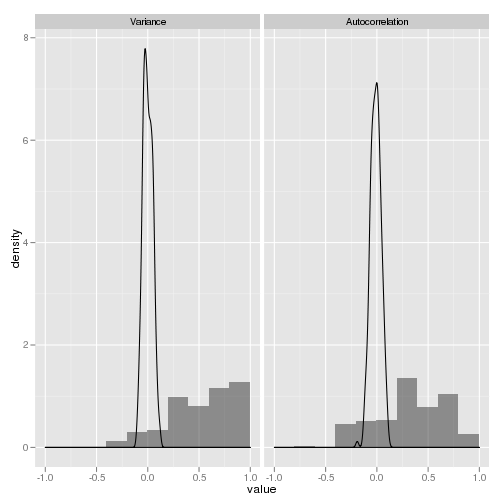
\includegraphics[width=.5\linewidth]{../appendix_fallacy/figure2.png}
\caption{Figure2}
\end{figure}


% BOILERPLATE - Allows for individual chapters to be compiled.
%
% Usage:
%    % BOILERPLATE - Allows for individual chapters to be compiled.
%
% Usage:
%    % BOILERPLATE - Allows for individual chapters to be compiled.
%
% Usage:
%    \input{../settings/boilerplate} % place at start and end of chapter
% 

\def\precommands{%
    \input{../settings/phdsetup}
    \def\preinserted{}
    \begin{document}
}

\def\postcommands{%
    \singlespacing
    \phantomsection
%    \bibliographystyle{../bibliography/expanded}
   \bibliographystyle{elsarticle-harv}
   \bibliography{../bibliography/references}
    \enddocument
}

\def\autoinsert{%
    \ifx\preinserted\undefined
        \expandafter\precommands
    \else
        \expandafter\postcommands
    \fi
}

\ifx\master\undefined\expandafter\autoinsert\fi

 % place at start and end of chapter
% 

\def\precommands{%
    % [ USER VARIABLES ]

\def\PHDTITLE {Regime shifts in ecology and evolution}
\def\PHDAUTHOR{Carl Boettiger}
\def\PHDSCHOOL{University of California, Davis}

\def\PHDMONTH {September}
\def\PHDYEAR  {2012}
\def\PHDDEPT {Center for Population Biology}

\def\BSSCHOOL {Princeton}
\def\BSYEAR   {2007}

\def\PHDCOMMITTEEA{Alan Hastings}
\def\PHDCOMMITTEEB{Peter Wainwright}
\def\PHDCOMMITTEEC{Brian Moore}

% [ GLOBAL SETUP ]

\documentclass[letterpaper,oneside,11pt]{report}


% [ CARL BOETTIGER`S CUSTOM COMMANDS, LIBRARIES, ETC ]

\usepackage{subfigure}
\usepackage[sort&compress]{natbib}
\usepackage{color}
\usepackage{fancyvrb}
\usepackage{ctable}


\usepackage{silence}
\WarningFilter{amsmath}{Underfull}     

%\newcommand{\argmax}{\operatorname{argmax}}
\newcommand{\ud}{\mathrm{d}}


\usepackage{calc}
\usepackage{breakcites}
\usepackage[newcommands]{ragged2e}
\usepackage{appendix}
\usepackage{comment}
\usepackage{xifthen}

\usepackage{graphicx}
\usepackage{epstopdf}


\renewenvironment{abstract}{\chapter*{Abstract}}{}
\renewcommand{\bibname}{Bibliography}
\renewcommand{\contentsname}{Table of Contents}

\makeatletter
\renewcommand{\@biblabel}[1]{\textsc{#1}}
\makeatother

% [ FONT SETTINGS ]

\usepackage[T1]{fontenc}
\usepackage{libertine}

\usepackage[tbtags, intlimits, namelimits]{amsmath}
\usepackage{amsthm}
\usepackage{amssymb}
\usepackage{amsfonts}



% [ PAGE LAYOUT ]

\usepackage{geometry}
\geometry{lmargin = 1.5in}
\geometry{rmargin = 1.0in}
\geometry{tmargin = 1.0in}
\geometry{bmargin = 1.0in}

% [ PDF SETTINGS ]

\usepackage[final]{hyperref}
\hypersetup{
    breaklinks  = {true},
    colorlinks  = {true},
    linktocpage = {false},
    linkcolor   = {blue},
    citecolor   = {black},
    urlcolor    = {black},
    plainpages  = {false},
    pageanchor  = {true},
    pdfauthor   = {\PHDAUTHOR},
    pdftitle    = {\PHDTITLE},
    pdfsubject  = {Dissertation, \PHDSCHOOL},
    pdfcreator  = {},
    pdfkeywords = {},
    pdfproducer = {}
}
\urlstyle{same}

% [ LETTER SPACING ]

\usepackage[final]{microtype}
\microtypesetup{protrusion=compatibility}
\microtypesetup{expansion=false}

\newcommand{\upper}[1]{\MakeUppercase{#1}}
\let\lsscshape\scshape

\ifcase\pdfoutput\else\microtypesetup{letterspace=15}
\renewcommand{\scshape}{\lsscshape\lsstyle}
\renewcommand{\upper}[1]{\textls[50]{\MakeUppercase{#1}}}\fi

% [ LINE SPACING ]

\usepackage[doublespacing]{setspace}
\renewcommand{\displayskipstretch}{0.75}

\setlength{\parskip   }{0em}
\setlength{\parindent }{2em}

% [ TABLE FORMATTING ]

\usepackage{booktabs}
\usepackage{multirow}
\usepackage{dcolumn}
\setlength{\heavyrulewidth}{1.5\arrayrulewidth}
\setlength{\lightrulewidth}{1.0\arrayrulewidth}
\setlength{\doublerulesep }{2.0\arrayrulewidth}

% [ SECTION FORMATTING ]

\usepackage[largestsep,nobottomtitles*]{titlesec}
\renewcommand{\bottomtitlespace}{0.75in}

\titleformat{\chapter}[display]%
    {\bfseries\huge\singlespacing}%
    {\filleft\textsc{\LARGE \chaptertitlename\ \thechapter}}%
    {-0.2ex}{\titlerule[3pt]\vspace{0.2ex}}[]

\titleformat{\section}{\LARGE}{\thesection\hspace{0.5em}}{0ex}{}
\titleformat{\subsection}{\Large}{\thesubsection\hspace{0.5em}}{0ex}{}
\titleformat{\subsubsection}{\large}{\thesubsubsection\hspace{0.5em}}{0ex}{}

\titlespacing*{\chapter}{0em}{6ex}{4ex plus 2ex minus 0ex}
\titlespacing*{\section}{0em}{2ex plus 3ex minus 1ex}{0.5ex plus 0.5ex minus 0.5ex}
\titlespacing*{\subsection}{0ex}{2ex plus 3ex minus 1ex}{0ex}
\titlespacing*{\subsubsection}{0ex}{2ex plus 0ex minus 1ex}{0ex}

% [ HEADER SETTINGS ]

\usepackage{fancyhdr}

\setlength{\headheight}{\normalbaselineskip}
\setlength{\footskip  }{0.5in}
\setlength{\headsep   }{0.5in-\headheight}

\fancyheadoffset[R]{0.5in}
\renewcommand{\headrulewidth}{0pt}
\renewcommand{\footrulewidth}{0pt}

\newcommand{\pagebox}{\parbox[r][\headheight][t]{0.5in}{\hspace\fill\thepage}}

\newcommand{\prelimheaders}{\ifx\prelim\undefined\renewcommand{\thepage}{\textit{\roman{page}}}\fancypagestyle{plain}{\fancyhf{}\fancyfoot[L]{\makebox[\textwidth-0.5in]{\thepage}}}\pagestyle{plain}\def\prelim{}\fi}

\newcommand{\normalheaders}{\renewcommand{\thepage}{\arabic{page}}\fancypagestyle{plain}{\fancyhf{}\fancyhead[R]{\pagebox}}\pagestyle{plain}}

\normalheaders{}

% [ CUSTOM COMMANDS ]

\newcommand{\signaturebox}[1]{\multicolumn{1}{p{4in}}{\vspace{3ex}}\\\midrule #1\\}

% Redefine AMS proof environment to have itshape
% Note: This environment automatically adds \qed at the end. If your proof
% ends in a math environment, the \qed is placed, undesirably, on a new line.
% To prevent that, insert \qedhere inside the math environment.
\makeatletter
\renewenvironment{proof}[1][\proofname]{%
\par\pushQED{\qed}\normalfont%
\topsep6\p@\@plus6\p@\relax\trivlist%
\item[\hskip\labelsep\bfseries#1\@addpunct{.}]\itshape\ignorespaces}{%
\popQED\endtrivlist\@endpefalse}%
\makeatother

% TUGboat, Volume 0 (2001), No. 0
% http://math.arizona.edu/~aprl/publications/mathclap/perlis_mathclap_24Jun2003.pdf
% For comparison, here are the existing overlap macros:
% \def\llap#1{\hbox to 0pt{\hss#1}}
% \def\rlap#1{\hbox to 0pt{#1\hss}}
\def\clap#1{\hbox to 0pt{\hss#1\hss}}
\def\mathllap{\mathpalette\mathllapinternal}
\def\mathrlap{\mathpalette\mathrlapinternal}
\def\mathclap{\mathpalette\mathclapinternal}
\def\mathllapinternal#1#2{%
\llap{$\mathsurround=0pt#1{#2}$}}
\def\mathrlapinternal#1#2{%
\rlap{$\mathsurround=0pt#1{#2}$}}
\def\mathclapinternal#1#2{%
\clap{$\mathsurround=0pt#1{#2}$}}

\newcommand{\alert}[1]{\textbf{\textcolor{red}{#1}}}




% [ Code blocks ]
%\DefineShortVerb[commandchars=\\\{\}]{\|}
\DefineVerbatimEnvironment{Highlighting}{Verbatim}{commandchars=\\\{\}}
% Add ',fontsize=\small' for more characters per line
\newenvironment{Shaded}{}{}
\newcommand{\KeywordTok}[1]{\textcolor[rgb]{0.00,0.44,0.13}{\textbf{{#1}}}}
\newcommand{\DataTypeTok}[1]{\textcolor[rgb]{0.56,0.13,0.00}{{#1}}}
\newcommand{\DecValTok}[1]{\textcolor[rgb]{0.25,0.63,0.44}{{#1}}}
\newcommand{\BaseNTok}[1]{\textcolor[rgb]{0.25,0.63,0.44}{{#1}}}
\newcommand{\FloatTok}[1]{\textcolor[rgb]{0.25,0.63,0.44}{{#1}}}
\newcommand{\CharTok}[1]{\textcolor[rgb]{0.25,0.44,0.63}{{#1}}}
\newcommand{\StringTok}[1]{\textcolor[rgb]{0.25,0.44,0.63}{{#1}}}
\newcommand{\CommentTok}[1]{\textcolor[rgb]{0.38,0.63,0.69}{\textit{{#1}}}}
\newcommand{\OtherTok}[1]{\textcolor[rgb]{0.00,0.44,0.13}{{#1}}}
\newcommand{\AlertTok}[1]{\textcolor[rgb]{1.00,0.00,0.00}{\textbf{{#1}}}}
\newcommand{\FunctionTok}[1]{\textcolor[rgb]{0.02,0.16,0.49}{{#1}}}
\newcommand{\RegionMarkerTok}[1]{{#1}}
\newcommand{\ErrorTok}[1]{\textcolor[rgb]{1.00,0.00,0.00}{\textbf{{#1}}}}
\newcommand{\NormalTok}[1]{{#1}}



    \def\preinserted{}
    \begin{document}
}

\def\postcommands{%
    \singlespacing
    \phantomsection
%    \bibliographystyle{../bibliography/expanded}
   \bibliographystyle{elsarticle-harv}
   \bibliography{../bibliography/references}
    \enddocument
}

\def\autoinsert{%
    \ifx\preinserted\undefined
        \expandafter\precommands
    \else
        \expandafter\postcommands
    \fi
}

\ifx\master\undefined\expandafter\autoinsert\fi

 % place at start and end of chapter
% 

\def\precommands{%
    % [ USER VARIABLES ]

\def\PHDTITLE {Regime shifts in ecology and evolution}
\def\PHDAUTHOR{Carl Boettiger}
\def\PHDSCHOOL{University of California, Davis}

\def\PHDMONTH {September}
\def\PHDYEAR  {2012}
\def\PHDDEPT {Center for Population Biology}

\def\BSSCHOOL {Princeton}
\def\BSYEAR   {2007}

\def\PHDCOMMITTEEA{Alan Hastings}
\def\PHDCOMMITTEEB{Peter Wainwright}
\def\PHDCOMMITTEEC{Brian Moore}

% [ GLOBAL SETUP ]

\documentclass[letterpaper,oneside,11pt]{report}


% [ CARL BOETTIGER`S CUSTOM COMMANDS, LIBRARIES, ETC ]

\usepackage{subfigure}
\usepackage[sort&compress]{natbib}
\usepackage{color}
\usepackage{fancyvrb}
\usepackage{ctable}


\usepackage{silence}
\WarningFilter{amsmath}{Underfull}     

%\newcommand{\argmax}{\operatorname{argmax}}
\newcommand{\ud}{\mathrm{d}}


\usepackage{calc}
\usepackage{breakcites}
\usepackage[newcommands]{ragged2e}
\usepackage{appendix}
\usepackage{comment}
\usepackage{xifthen}

\usepackage{graphicx}
\usepackage{epstopdf}


\renewenvironment{abstract}{\chapter*{Abstract}}{}
\renewcommand{\bibname}{Bibliography}
\renewcommand{\contentsname}{Table of Contents}

\makeatletter
\renewcommand{\@biblabel}[1]{\textsc{#1}}
\makeatother

% [ FONT SETTINGS ]

\usepackage[T1]{fontenc}
\usepackage{libertine}

\usepackage[tbtags, intlimits, namelimits]{amsmath}
\usepackage{amsthm}
\usepackage{amssymb}
\usepackage{amsfonts}



% [ PAGE LAYOUT ]

\usepackage{geometry}
\geometry{lmargin = 1.5in}
\geometry{rmargin = 1.0in}
\geometry{tmargin = 1.0in}
\geometry{bmargin = 1.0in}

% [ PDF SETTINGS ]

\usepackage[final]{hyperref}
\hypersetup{
    breaklinks  = {true},
    colorlinks  = {true},
    linktocpage = {false},
    linkcolor   = {blue},
    citecolor   = {black},
    urlcolor    = {black},
    plainpages  = {false},
    pageanchor  = {true},
    pdfauthor   = {\PHDAUTHOR},
    pdftitle    = {\PHDTITLE},
    pdfsubject  = {Dissertation, \PHDSCHOOL},
    pdfcreator  = {},
    pdfkeywords = {},
    pdfproducer = {}
}
\urlstyle{same}

% [ LETTER SPACING ]

\usepackage[final]{microtype}
\microtypesetup{protrusion=compatibility}
\microtypesetup{expansion=false}

\newcommand{\upper}[1]{\MakeUppercase{#1}}
\let\lsscshape\scshape

\ifcase\pdfoutput\else\microtypesetup{letterspace=15}
\renewcommand{\scshape}{\lsscshape\lsstyle}
\renewcommand{\upper}[1]{\textls[50]{\MakeUppercase{#1}}}\fi

% [ LINE SPACING ]

\usepackage[doublespacing]{setspace}
\renewcommand{\displayskipstretch}{0.75}

\setlength{\parskip   }{0em}
\setlength{\parindent }{2em}

% [ TABLE FORMATTING ]

\usepackage{booktabs}
\usepackage{multirow}
\usepackage{dcolumn}
\setlength{\heavyrulewidth}{1.5\arrayrulewidth}
\setlength{\lightrulewidth}{1.0\arrayrulewidth}
\setlength{\doublerulesep }{2.0\arrayrulewidth}

% [ SECTION FORMATTING ]

\usepackage[largestsep,nobottomtitles*]{titlesec}
\renewcommand{\bottomtitlespace}{0.75in}

\titleformat{\chapter}[display]%
    {\bfseries\huge\singlespacing}%
    {\filleft\textsc{\LARGE \chaptertitlename\ \thechapter}}%
    {-0.2ex}{\titlerule[3pt]\vspace{0.2ex}}[]

\titleformat{\section}{\LARGE}{\thesection\hspace{0.5em}}{0ex}{}
\titleformat{\subsection}{\Large}{\thesubsection\hspace{0.5em}}{0ex}{}
\titleformat{\subsubsection}{\large}{\thesubsubsection\hspace{0.5em}}{0ex}{}

\titlespacing*{\chapter}{0em}{6ex}{4ex plus 2ex minus 0ex}
\titlespacing*{\section}{0em}{2ex plus 3ex minus 1ex}{0.5ex plus 0.5ex minus 0.5ex}
\titlespacing*{\subsection}{0ex}{2ex plus 3ex minus 1ex}{0ex}
\titlespacing*{\subsubsection}{0ex}{2ex plus 0ex minus 1ex}{0ex}

% [ HEADER SETTINGS ]

\usepackage{fancyhdr}

\setlength{\headheight}{\normalbaselineskip}
\setlength{\footskip  }{0.5in}
\setlength{\headsep   }{0.5in-\headheight}

\fancyheadoffset[R]{0.5in}
\renewcommand{\headrulewidth}{0pt}
\renewcommand{\footrulewidth}{0pt}

\newcommand{\pagebox}{\parbox[r][\headheight][t]{0.5in}{\hspace\fill\thepage}}

\newcommand{\prelimheaders}{\ifx\prelim\undefined\renewcommand{\thepage}{\textit{\roman{page}}}\fancypagestyle{plain}{\fancyhf{}\fancyfoot[L]{\makebox[\textwidth-0.5in]{\thepage}}}\pagestyle{plain}\def\prelim{}\fi}

\newcommand{\normalheaders}{\renewcommand{\thepage}{\arabic{page}}\fancypagestyle{plain}{\fancyhf{}\fancyhead[R]{\pagebox}}\pagestyle{plain}}

\normalheaders{}

% [ CUSTOM COMMANDS ]

\newcommand{\signaturebox}[1]{\multicolumn{1}{p{4in}}{\vspace{3ex}}\\\midrule #1\\}

% Redefine AMS proof environment to have itshape
% Note: This environment automatically adds \qed at the end. If your proof
% ends in a math environment, the \qed is placed, undesirably, on a new line.
% To prevent that, insert \qedhere inside the math environment.
\makeatletter
\renewenvironment{proof}[1][\proofname]{%
\par\pushQED{\qed}\normalfont%
\topsep6\p@\@plus6\p@\relax\trivlist%
\item[\hskip\labelsep\bfseries#1\@addpunct{.}]\itshape\ignorespaces}{%
\popQED\endtrivlist\@endpefalse}%
\makeatother

% TUGboat, Volume 0 (2001), No. 0
% http://math.arizona.edu/~aprl/publications/mathclap/perlis_mathclap_24Jun2003.pdf
% For comparison, here are the existing overlap macros:
% \def\llap#1{\hbox to 0pt{\hss#1}}
% \def\rlap#1{\hbox to 0pt{#1\hss}}
\def\clap#1{\hbox to 0pt{\hss#1\hss}}
\def\mathllap{\mathpalette\mathllapinternal}
\def\mathrlap{\mathpalette\mathrlapinternal}
\def\mathclap{\mathpalette\mathclapinternal}
\def\mathllapinternal#1#2{%
\llap{$\mathsurround=0pt#1{#2}$}}
\def\mathrlapinternal#1#2{%
\rlap{$\mathsurround=0pt#1{#2}$}}
\def\mathclapinternal#1#2{%
\clap{$\mathsurround=0pt#1{#2}$}}

\newcommand{\alert}[1]{\textbf{\textcolor{red}{#1}}}




% [ Code blocks ]
%\DefineShortVerb[commandchars=\\\{\}]{\|}
\DefineVerbatimEnvironment{Highlighting}{Verbatim}{commandchars=\\\{\}}
% Add ',fontsize=\small' for more characters per line
\newenvironment{Shaded}{}{}
\newcommand{\KeywordTok}[1]{\textcolor[rgb]{0.00,0.44,0.13}{\textbf{{#1}}}}
\newcommand{\DataTypeTok}[1]{\textcolor[rgb]{0.56,0.13,0.00}{{#1}}}
\newcommand{\DecValTok}[1]{\textcolor[rgb]{0.25,0.63,0.44}{{#1}}}
\newcommand{\BaseNTok}[1]{\textcolor[rgb]{0.25,0.63,0.44}{{#1}}}
\newcommand{\FloatTok}[1]{\textcolor[rgb]{0.25,0.63,0.44}{{#1}}}
\newcommand{\CharTok}[1]{\textcolor[rgb]{0.25,0.44,0.63}{{#1}}}
\newcommand{\StringTok}[1]{\textcolor[rgb]{0.25,0.44,0.63}{{#1}}}
\newcommand{\CommentTok}[1]{\textcolor[rgb]{0.38,0.63,0.69}{\textit{{#1}}}}
\newcommand{\OtherTok}[1]{\textcolor[rgb]{0.00,0.44,0.13}{{#1}}}
\newcommand{\AlertTok}[1]{\textcolor[rgb]{1.00,0.00,0.00}{\textbf{{#1}}}}
\newcommand{\FunctionTok}[1]{\textcolor[rgb]{0.02,0.16,0.49}{{#1}}}
\newcommand{\RegionMarkerTok}[1]{{#1}}
\newcommand{\ErrorTok}[1]{\textcolor[rgb]{1.00,0.00,0.00}{\textbf{{#1}}}}
\newcommand{\NormalTok}[1]{{#1}}



    \def\preinserted{}
    \begin{document}
}

\def\postcommands{%
    \singlespacing
    \phantomsection
%    \bibliographystyle{../bibliography/expanded}
   \bibliographystyle{elsarticle-harv}
   \bibliography{../bibliography/references}
    \enddocument
}

\def\autoinsert{%
    \ifx\preinserted\undefined
        \expandafter\precommands
    \else
        \expandafter\postcommands
    \fi
}

\ifx\master\undefined\expandafter\autoinsert\fi



